\documentclass{article}
\usepackage[paperwidth=6cm, paperheight=6cm, margin = 0cm, top=0.5cm]{geometry}
\usepackage{amsmath}


\usepackage{pgf}
\usepackage{tikz}


\usetikzlibrary{arrows,automata}

\tikzstyle{source}  = [draw,circle,fill=black,thick,inner sep=0mm,minimum size=2mm]

\renewcommand{\vec}[1]{\boldsymbol{#1}}

\begin{document}
\begin{center}
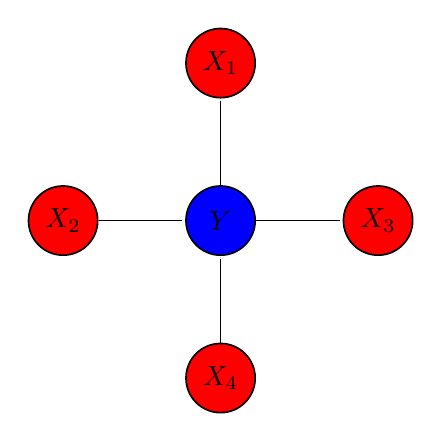
\begin{tikzpicture}[-,>=stealth',shorten >=1pt,auto,node distance=2cm,semithick]
                    

\node[state, fill=blue] (Y3) {$Y$}; 
\node[state, fill=red]  (Z3) [above of=Y3] {$X_{1}$}; 
\node[state, fill=red]  (Y4) [right of=Y3] {$X_{3}$}; 
\node[state, fill=red]  (Y2) [left  of=Y3] {$X_{2}$}; 
\node[state, fill=red]  (X3) [below of=Y3] {$X_{4}$};                   

	
\path
	(Y2) edge (Y3)
	(Y3) edge (Y4);

\path	
	(X3) edge (Y3);
\path	
	(Y3) edge (Z3);




\end{tikzpicture}
\end{center}

\end{document}
